\documentclass{article}
\usepackage[utf8]{inputenc}
\usepackage{fullpage}
\usepackage{amsmath}
\usepackage{graphicx}
\graphicspath{ {./images/} }

\title{Feynman's Technique for Computing Integrals}
\author{Tyler Lin}
\date{January 2020}

\begin{document}

\maketitle

\section*{Problem 1}
Compute the daunting integral $$\int_{0}^{\pi} \ln(1-2\alpha\cos{x}+\alpha^2)dx$$ for $|\alpha|<1$.
\newline We can try the usual tricks, starting with trig substitution:
$$\alpha=\tan{\theta}$$
$$1+\alpha^2=1+\tan^2{\theta}=\sec^2{\theta}$$
So the integral reduces to $$\int_{0}^{\pi} \ln(\sec^2{\theta}-2\tan{\theta}\cos{x})dx$$ for $|\theta| \in [0,\pi/4) \cup (3\pi/4, \pi]$.
Perhaps integration by parts shall suffice.
$$u=\ln(\sec^2{\theta}-2\tan{\theta}\cos{x}) \hspace{10mm} dv=dx$$
$$du=\frac{2\tan{\theta}\sin{x}}{\sec^2{\theta}-2\tan{\theta}\cos{x}}dx \hspace{10mm} v=x$$
We now have
$$x\ln(\sec^2{\theta}-2\tan{\theta}\cos{x})\bigg\vert_{0}^{\pi} - \int_{0}^{\pi} \frac{2x\tan{\theta}\sin{x}}{\sec^2{\theta}-2\tan{\theta}\cos{x}}dx$$
$$= \pi\ln(\sec^2{\theta}+2\tan{\theta}) - \int_{0}^{\pi} \frac{2x\tan{\theta}\sin{x}}{\sec^2{\theta}-2\tan{\theta}\cos{x}}dx,$$
where $|\theta| \in [0,\pi/4) \cup (3\pi/4, \pi]$.
\newline I shall leave it to the reader to try to decipher the rightmost integral if they wish, but I hope they take my word that they will be unable to find a solution. Note that everything involving $\theta$ is a constant.
\newline I do not wish to digress too far from the main topic of this paper, which is solving the given integral using Feynman's technique. Just to be sure Feynman's technique is the only solution, let's try using integration by parts as the first step. 
$$u=\ln(1-2\alpha\cos{x}+\alpha^2) \hspace{10mm} dv=dx$$
$$du=\frac{2\alpha\sin{x}}{1-2\alpha\cos{x}+\alpha^2}dx \hspace{10mm} v=x$$
We are left with
$$x\ln(1-2\alpha\cos{x}+\alpha^2)\bigg\vert_{0}^{\pi} - \int_{0}^{\pi}\frac{2\alpha{x}\sin{x}}{1-2\alpha\cos{x}+\alpha^2}dx$$
$$= \pi\ln(1+2\alpha+\alpha^2) - \int_{0}^{\pi}\frac{2\alpha{x}\sin{x}}{1-2\alpha\cos{x}+\alpha^2}dx,$$
where $|\alpha|<1$. 
\newline Again the reader may try solving the rightmost integral if he/she wishes, but a solution will not be reached. In fact, any method that the reader tries besides Feynman's technique, whether it be change of variable, series, or even Wolfram Alpha, will not result in a solution.

\section*{The Solution (using Feynman's Technique)}
\newline Now we get to the good stuff. Richard Feynman was a renowned American theoretical physicist. His technique for solving integrals was known as \textbf{Feynman's Technique}, but he really learned it from a book he read in high school, \textit{Advanced Calculus}, published in 1926 by MIT mathematician Frederick S. Woods. The original name of the technique is the \textbf{Leibniz Integral Rule}, and the given integral originates from that book. However, I will refer to the rule with the popularized name.
\subsection*{How Feynman's Technique Works}
Note that $\alpha$ is simply a constant with respect to the integral, so we can treat the integral itself as a function of $\alpha$.
$$\text{Let } f(\alpha)=\int_{0}^{\pi} \ln(1-2\alpha\cos{x}+\alpha^2)dx.$$
Next, we evaluate an $\alpha$ that gives us a convenient output. In this case it is when $\alpha=1$.
$$f(1)=\int_{0}^{\pi} \ln(2-2\cos{x})dx.$$
This ends up being
$$-\frac{3\pi\ln{4}-i\pi^2}{3}+\pi\ln{4}-\frac{i\pi^2}{3} = 0,$$
so $f(1)=0.$ This will be used in the final step.
\newline Here is the crucial step: we differentiate the integral with respect to alpha.
$$\frac{\partial f}{\partial \alpha} = \int_{0}^{\pi}\frac{\partial}{\partial \alpha}\ln(1-2\alpha\cos{x}+\alpha^2)dx = \int_{0}^{\pi}\frac{-2\cos{x}+2\alpha}{1-2\alpha\cos{x}+\alpha^2}dx$$
While this looks messy, and similar to what we got above, this is solvable.
$$\int_{0}^{\pi}\frac{-2\cos{x}+2\alpha}{1-2\alpha\cos{x}+\alpha^2}dx = \frac{1}{\alpha}\int_{0}^{\pi}\frac{-2\alpha\cos{x}+2\alpha^2}{1-2\alpha\cos{x}+\alpha^2}dx = \frac{1}{\alpha}\int_{0}^{\pi}\frac{-2\alpha\cos{x}+2\alpha^2}{1-2\alpha\cos{x}+\alpha^2}dx - 1 + 1$$
$$=\frac{1}{\alpha}\int_{0}^{\pi}\frac{-2\alpha\cos{x}+2\alpha^2}{1-2\alpha\cos{x}+\alpha^2}dx - \frac{1-2\alpha\cos{x}+\alpha^2}{1-2\alpha\cos{x}+\alpha^2} + 1$$
$$=\frac{1}{\alpha}\int_{0}^{\pi}\frac{\alpha^2-1}{1-2\alpha\cos{x}+\alpha^2} + 1 = \frac{1}{\alpha}\int_{0}^{\pi}1 - \frac{1-\alpha^2}{1-2\alpha\cos{x}+\alpha^2}$$
Dividing everything by $1+\alpha^2$, we get
$$\frac{\partial f}{\partial \alpha} = \frac{1}{\alpha}(\pi-\frac{1-\alpha^2}{1+\alpha^2})\int_{0}^{\pi}\frac{1}{1-\frac{2\alpha}{1+\alpha^2}\cos{x}}dx,$$
so
\begin{equation}
    \frac{\partial f}{\partial \alpha} = \frac{\pi}{\alpha}-(\frac{1}{\alpha})(\frac{1-\alpha^2}{1+\alpha^2})\int_{0}^{\pi}\frac{1}{1-\frac{2\alpha}{1+\alpha^2}\cos{x}}dx
\end{equation}
Finally, the rightmost integral is solve-able! We use a reverse $u$ substitution: Let $x=2\arctan{u}$. Then $\cos{x}=\frac{1-u^2}{1+u^2}$, $u=\tan{\frac{x}{2}}$, and $dx=\frac{2du}{1+u^2}$.
$$\int_{0}^{\pi}\frac{1}{1-\frac{2\alpha}{1+\alpha^2}\cos{x}}dx = \int_{0}^{\pi}\frac{2du}{1-\frac{2\alpha}{1+\alpha^2}\frac{1-u^2}{1+u^2}}$$
$$= \int_{0}^{\pi}\frac{2du}{1+u^2-\frac{2\alpha(1-u^2)}{1+\alpha^2}} = \int_{0}^{\pi}\frac{2(1+\alpha^2)du}{(1+u^2)(1+\alpha^2)-2\alpha(1-u^2)}$$
$$= \int_{0}^{\pi}\frac{2(1+\alpha^2)du}{1+u^2+\alpha^2+u^2\alpha^2-2\alpha+2\alpha u^2} = \int_{0}^{\pi}\frac{2(1+\alpha^2)du}{1-2\alpha+\alpha^2+u^2(1+2\alpha+\alpha^2)}$$
$$= \int_{0}^{\pi}\frac{2(1+\alpha^2)du}{(1-\alpha)^2+(1+\alpha)^2u^2} = \frac{2(1+\alpha^2)}{(1-\alpha)^2}\int_{0}^{\pi}\frac{du}{1+(\frac{1+\alpha}{1-\alpha})^2u^2}$$
Note that $\frac{1+\alpha}{1-\alpha}$ ranges from 0 to $-\infty$ because $|\alpha|<1$. Therefore if we denote the constant $\beta$ to be $$\beta=\frac{1+\alpha}{1-\alpha}u \text{ and } d\beta=\frac{1+\alpha}{1-\alpha}du \text { (so } du=\frac{1-\alpha}{1+\alpha}d\beta \text{)},$$
$$\frac{2(1+\alpha^2)}{(1-\alpha)^2}\int_{0}^{\pi}\frac{du}{1+(\frac{1+\alpha}{1-\alpha})^2u^2} = \frac{2(1+\alpha^2)}{(1-\alpha)(1+\alpha)}\int_{0}^{-\infty}\frac{d\beta}{1+\beta^2}$$
This looks familiar!
$$= \frac{2(1+\alpha^2)}{1-\alpha^2}\arctan{\beta}\bigg\vert_{0}^{-\infty}$$
$$= \frac{2(1+\alpha^2)}{1-\alpha^2}(\frac{-\pi}{2}) = \frac{-\pi(1+\alpha^2)}{1-\alpha^2}.$$
The integral portion of equation (1) is now simplified, but we must not forget the other parts to finally solve for our differential equation with respect to $\alpha$.
$$\frac{\partial f}{\partial \alpha} = \frac{\pi}{\alpha}-(\frac{1}{\alpha})(\frac{1-\alpha^2}{1+\alpha^2})\frac{-\pi(1+\alpha^2)}{1-\alpha^2} = \frac{\pi}{\alpha}-\frac{-\pi}{\alpha} = \frac{2\pi}{\alpha}$$
We can now solve for $f(\alpha)$ by integrating.
$$f(\alpha) = 2\pi\ln{|\alpha|}+C$$
Using our previously obtained equation of $f(1)=0$,
$$f(1)=2\pi\ln{1}+C=0 \rightarrow C=0$$
Finishing up,
$$\int_{0}^{\pi} \ln(1-2\alpha\cos{x}+\alpha^2)dx \text{ for } |\alpha|<1 = f(\alpha) = \boxed{2\pi\ln(|\alpha|)}.$$ 
This technique of \textbf{differentiating under the integral sign} is obscure, but very powerful in certain situations. In this case, using Feynman's techique is by far the most simple solution. Here is another, simpler example.

\section*{Problem 2}
Evaluate $$\int_{0}^{1}\frac{x^2-1}{\log{x}}dx.$$
The integrand must have two values to apply Feynman's technique, so we introduce the constant $k$ such that
$$f(k) = \int_{0}^{1}\frac{x^k-1}{\log{x}}dx$$ for $k>0$. Now we must find a $k$ such that $f(k)$ is convenient. Logically, we start with $k=0$. 
$$f(0)=\int_{0}^{1}\frac{1-1}{\log{x}}dx = 0.$$
\newline We proceed with \textbf{differentiating under the integral sign}.
$$\frac{df}{dk} = \frac{d}{dk}\int_{0}^{1}\frac{x^k-1}{\log{x}}dx = \int_{0}^{1}\frac{\partial}{\partial k}\frac{x^k-1}{\log{x}}dx$$
$$= \int_{0}^{1}x^kdx = \frac{x^{k+1}}{k+1}\bigg\vert_{0}^{1} = \frac{1}{k+1}$$
Integrating,
$$f(k)=\ln({k+1})+C.$$
We know from previously that $f(0)=0$, and $f(0)=\ln(1)+C=0+C$, so $C=0$. Therefore to solve the original integral we calculate $f(2)$.
$$\int_{0}^{1}\frac{x^2-1}{\log{x}}dx = f(2) = \boxed{\log({3})}.$$

\section*{Exercises for the Reader}
The solution to these integrals are much shorter than the first example, so don't hesitate to try them.
\newline \newline 1. \textit{Use Feynman's technique to evaluate the following integral, $A5$ from the 2005 Putnam Competition}:
$$\int_{0}^{1}\frac{\ln(x+1)}{x^2+1}dx$$
2. \textit{Use Feynman's technique to evaluate}
$$\int_{0}^{\pi}e^{\cos{x}}\cos{(\sin{x})}dx.$$
The answers can be found on the next page. Happy integrating!

\newpage
\section*{Answers to Exercises}
1. $\boxed{\dfrac{\pi\ln{2}}{8}}$
\newline \textit{Hint}: Let $\displaystyle{f(k)=\int_{0}^{1}\frac{\ln({kx-1})}{x^2+1}}dx$
\newline \newline 2. $\boxed{0}$
\newline \textit{Hint}: Let $\displaystyle{f(k)=\int_{0}^{\pi}e^{k\cos{x}}\cos({k\sin{x}})}dx$
\begin{thebibliography}{2}
\bibitem{book}
Feynman, Richard P.
\textit{Surely You're Joking, Mr. Feynman!}
Bantam Books, 1986.

\bibitem{medium}
The Red, Panda. "Richard Feynman's Integral Trick." 
\textit{Medium}, 16 July 2018, medium.com/cantors-paradise/richard-feynmans-integral-trick-e7afae85e25c. Accessed 18 Jan. 2020.
\end{thebibliography}

\begin{center}
    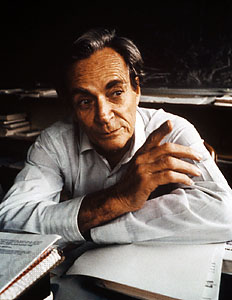
\includegraphics[scale=0.75]{feynman}
\end{center}
\end{document}